\chapter{Results}
	A model has been implemented which simulates 3 types of errors. The code has also been adapted to run on a computing cluster with multi-threading. This performance boost to the code allows for very large code sizes to be investigated, with multiple variables. Corroboration of results with literature has also been performed. Figure \ref{fig:unscaled} and figure \ref{fig:scaled} show how after the scaling factor in equation \ref{eq:scalingrelation} has been applied with $v_c = 1.49$ and $p_c = 0.103$, the various code sizes come into close agreement. These values agree with those determined by Stace and Barret \cite{Stace2010}, and Deutch et al \cite{Deutsch1985}.
	\\\\
	\begin{figure}[htpb]
	\begin{minipage}[t]{0.48\textwidth}
		\centering
		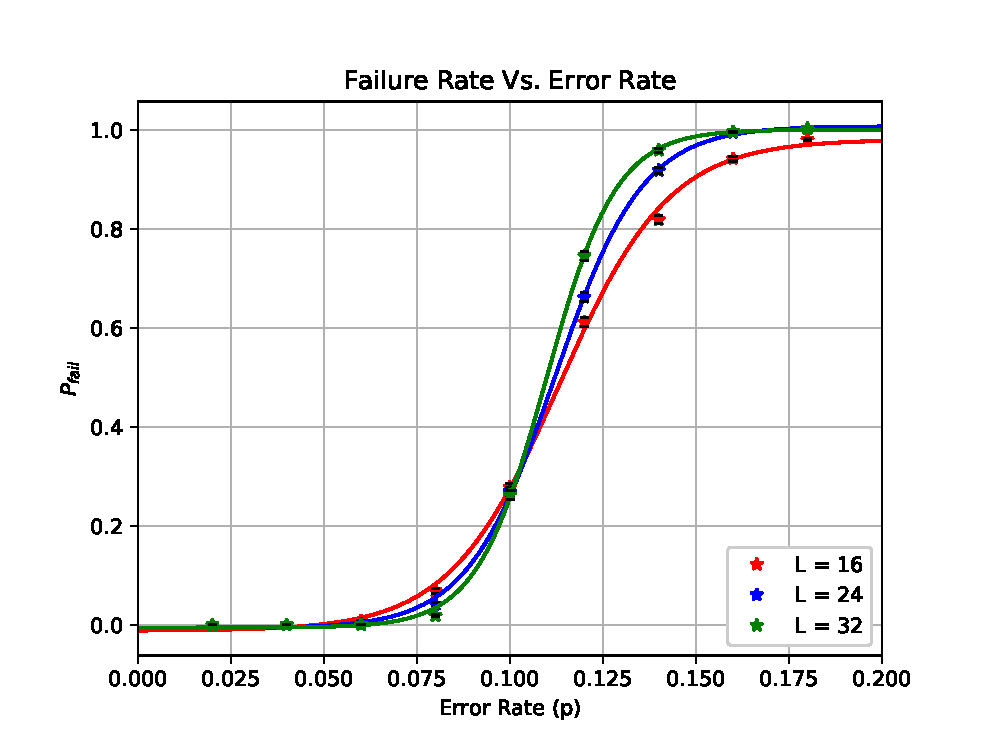
\includegraphics[width = \textwidth]{figs/unscaled.eps}
		\caption{This plot shows $P_{fail}$ Vs $p$ without any scaling applied, for 3 code sizes. A hyperbolic tangent trendline was fitted to allow the crossover point to be determined. Error bars have been plotted.}
		\label{fig:unscaled}
	\end{minipage}\hfill
	\begin{minipage}[t]{0.48\textwidth}
		\centering
			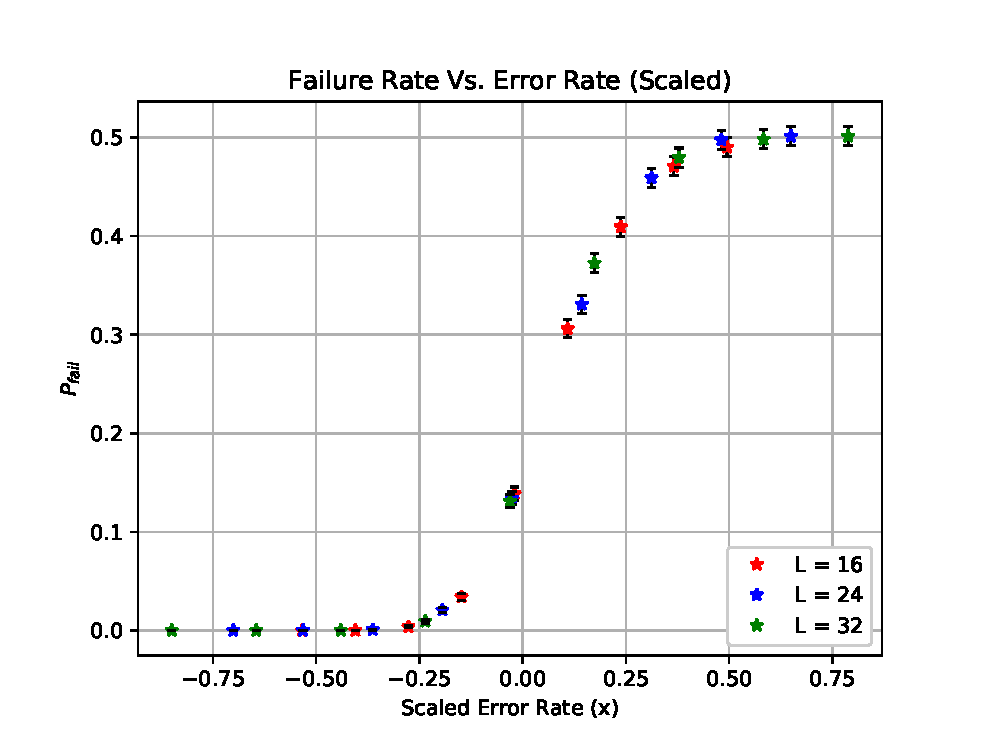
\includegraphics[width = \textwidth]{figs/scaled.eps}
			\caption{A plot of the rescaled data $x$ vs $P_{fail}$. $v_c = 1.49$, $p_c = 0.103$}
			\label{fig:scaled}
	\end{minipage}
	
	\end{figure}
	Data provided by figure \ref{fig:unscaled} determined $p_{c0}$ to be $0.103\pm 5$ ($10.3\pm 5 \%$ error), through the use of hyperbolic tangent trendlines.
\section{Correlated Errors}
\begin{figure}[htpb]
	\centering
	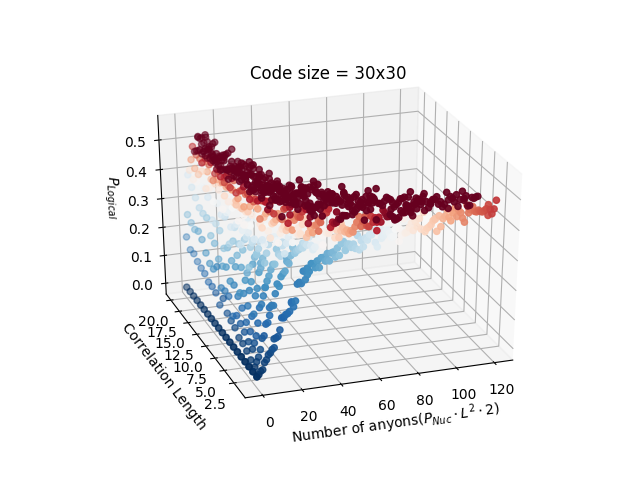
\includegraphics[width = 0.7\textwidth]{figs/30x30.png}
	\caption{A L=30 code with 5000 samples, showing both the effect of the number of error chains, and the length of those error chains on the success rate of the code.}
	\label{fig:3dplots}
\end{figure}
It can be seen in figure \ref{fig:3dplots} that the success rate of the code is dependant upon both the number of anyons and the chain length. It is also apparent that degree of correlation of errors has a distinct effect on the success rate, as these plots are not symmetric over the line of constant error rate. Figure \ref{fig:IncreasingCorr} shows that when the total number of errors is kept constant and the degree of correlation is increased, the failure rate of the code increases. 
\begin{figure}[htpb]
	\centering
	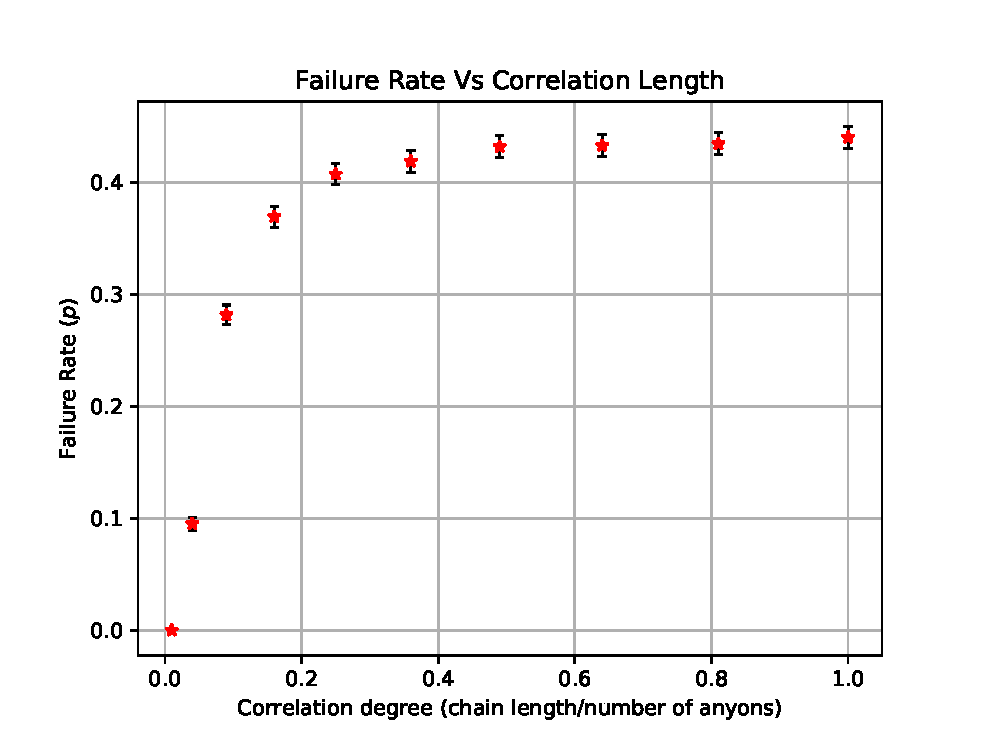
\includegraphics[scale = 0.7]{figs/pvscorr.eps}
	\caption{A 60x60 grid, with a constant number of error sites (11.1$\%$ of sites had error). This means that as the correlation length of the chains was increased, the number of chains was decreased, to keep the total number of affected sites constant. It can be seen that as the correlation length of the anyon gets longer, their failure rate increases; even with the total number of affected sites remaining constant. }
	\label{fig:IncreasingCorr}

\end{figure}


\section{Improved decoder}
initially we run the decoder with a variance of 1, and sweep the centre of th gaussian ($\overline{x}$) to determine if correcting for error correlations has any effect on the failure rate of the code. 
\begin{figure}[htpb]
	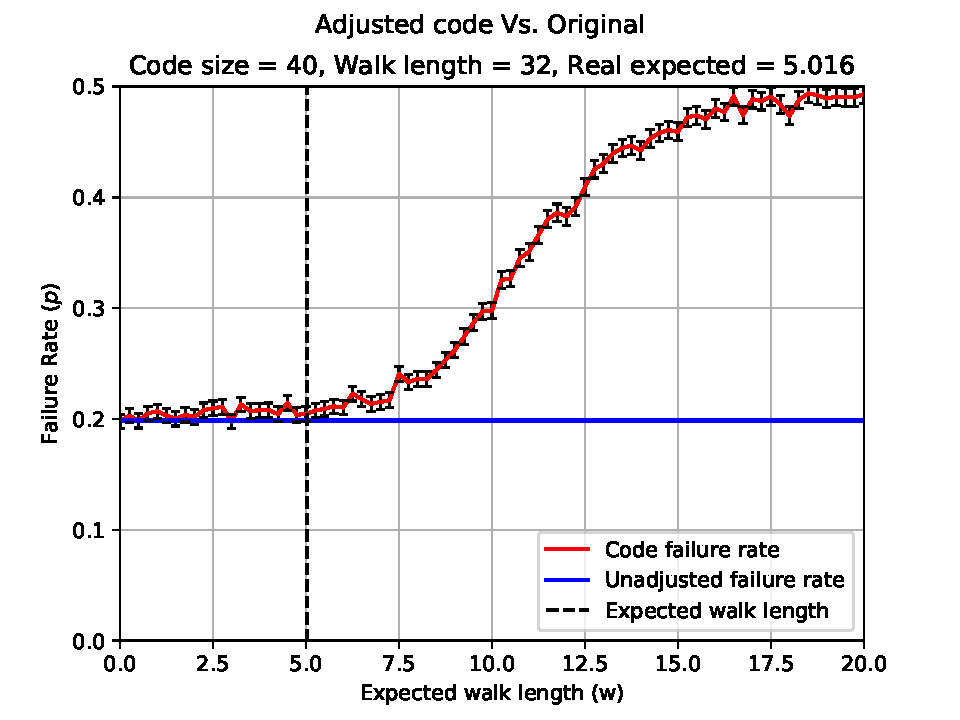
\includegraphics{figs/var1xbarvsfailure}
	\caption{this plot shows how the code implemented allows the code to match the failure rate of the origional code, even though it isnt least weight. this means that my code should work, with better parameters.}
	\label{fig:xbarplot1}
\end{figure}
Given that the adjusted code doesnt fail more than the origional code, up until a value close to the expected walk length predicted by all three methods, we shall use the a point near these predicted walk lengths to varying the next parameter in out gaussian, to attempt to improve the failure rate. 

Next we vary the variance ($\sigma^2$) of the gaussian correction, in an attempt to find an optimal value, so that we can again sweep over $\overline{x}$ to determine which distribution is the best to apply to reduce the failure rate further. 

\begin{figure}[htpb]
	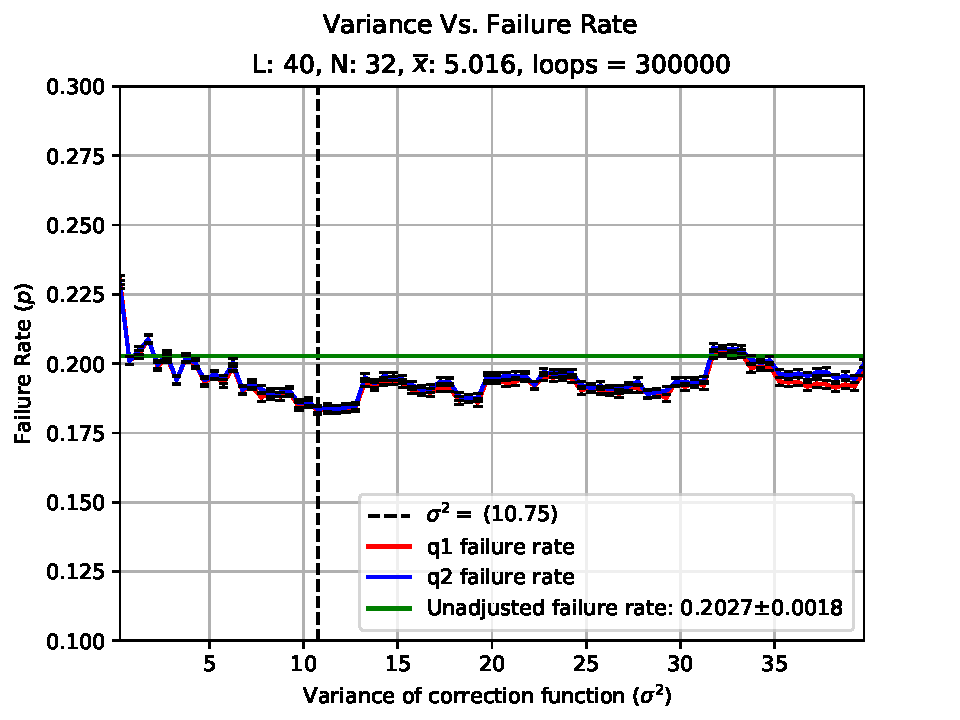
\includegraphics{figs/improvementl300000L40True_3398b43b399345d183a59bfda7727a61.pdf}
	\caption{This plot shows how the variance has a very interesting curve, for what variances can be optimal. This likely has effects/interactions from the other walks in locality. An optimal variance was found at $\sigma^2$ = 10.75. Variance was stepped in sizes of 0.5.}
	\label{fig:varplot}
\end{figure}
Figure \ref{fig:varplot} shows clearly how for certain variances, the improved decoder with gaussian walk length correction beats the least weight perfect matching algorithm used for uncorrelated errors. We will now used this value of 10.75 to perform a higher another run of sweeping $\overline{x}$ to determine which distribution/expected length's distribution should be most optimal. 




The first naive simulation we run is with a gaussian correction, to reduce the adjusted weight smaller near the RMS distance of the walk. Once we have good data from this, we shall then compare to the other distance methods to determine which is the best expected distance/distribution to use to design the optimal decoder. 

Using an expected walk length of 5.016, we vary the the variance of the 



\section{Correction schemes}

Two correction schemes were used to attempt to lower the failre rate. one method was a concatenation of the least weight linear relationship with a gaussian drop in distance close to the expected walk length. 
A THIRD CORRECTION SCHEME COULD BE TO CONCATENATE THE GAMMA FUNCTIONS WITH THE LINEAR SCALING SAME AS FOR THE RAW GAMMA FUNCTION


the other method was to determine the actual distribution of walk lengths, and reduce the distance of syndrome measurements accordingly.

\begin{figure}[htpb]
	\centering
	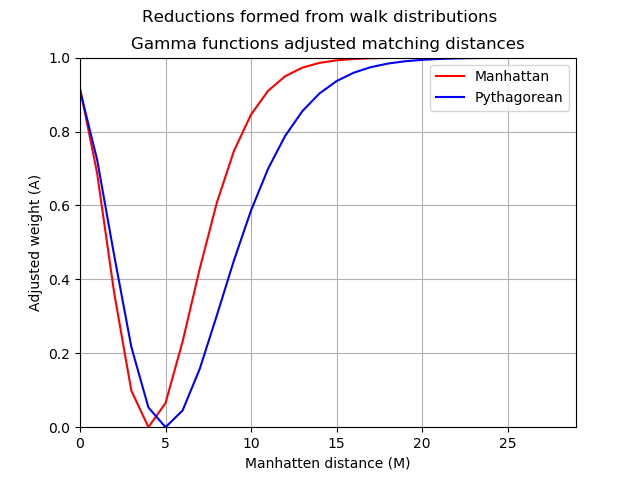
\includegraphics[width= 0.5\textwidth]{figs/gamma_corrections.png}
	\caption{this is how the distances were reduces accoring to the distributions}
	\label{fig:gamma}
\end{figure}
as canbe seen in \ref{fig:gamma} the distributions were adjusted to a peak height of unity, and were then inverted, to reduce the distances near the expected walk length. The distribution needed to be extended beyond the point of N as neighbouring walks can have a larger distance. The max distance should be sqrt(2*L*L)/2 +1 as this is the largest possible disagonal distance on the torus. 
\begin{itemize}
	\item generate x random walks 
	\item calculate gamma function parameters from this distribution
	\item calulate gaussian
	\item flip and create new weighting function
	\item apply for y code simulations and determine new failure rates
\end{itemize}

\section{Performance of Gaussian Correction}

\begin{figure}[htpb]
\centering
	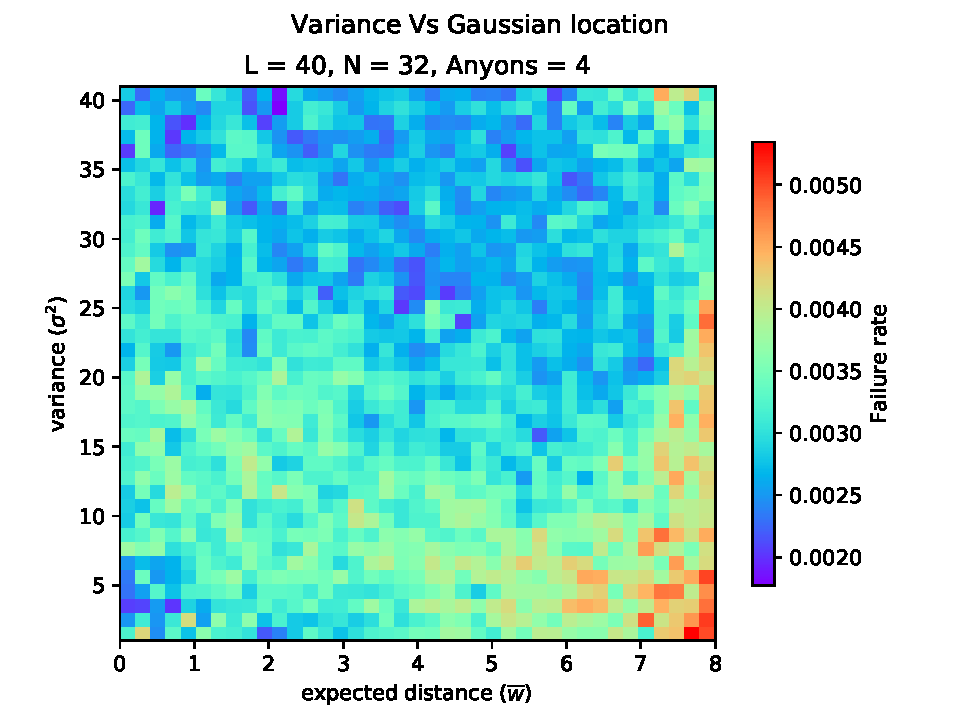
\includegraphics[width = 0.7\textwidth]{figs/A4N32l40000.pdf}
\caption{This figure shows the performance of the gaussian correction for $\sigma^2$ and $\overline{w}$ when 4 anyons are present with N=32 on a L=40 code.}
\label{fig:A4rough}
\end{figure}

Figure \ref{fig:A4rough} shows a similar trend to other anyon densities. However, even with 40,000 loops per point, the error rate is so low ($\overline{p} = 0.00314\pm 0.00002$) that resolving dependence on variables is difficult, as it becomes computationally difficult to reduce relative errors at this rate. For this reason higher numbers of anyons are primarily studied to decrease computation time.

\begin{figure}
\centering
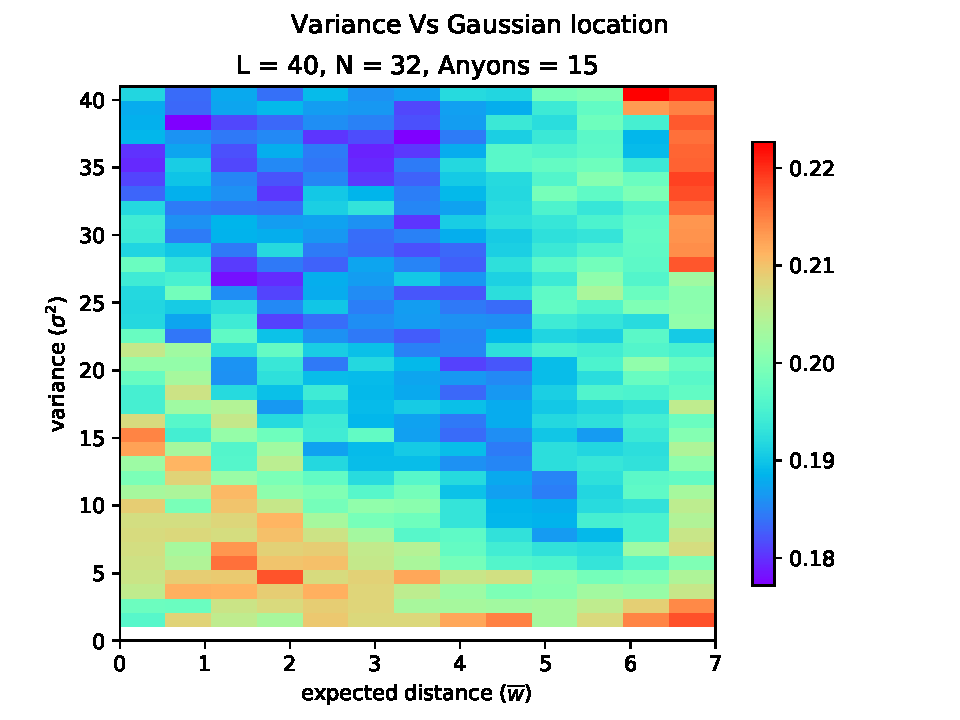
\includegraphics[width = 0.7\textwidth]{figs/variancevslocation_combined.pdf}
\caption{A large range scan of N=32 A=15 for $\sigma^2$ and $\overline{w}$}
\label{fig:A15rough}
\end{figure}
The variance was studied to very large values ($\sigma^2 = 40$) and a trend seems to form. As the variance is increased, the `best' $\overline{w}$ also walks up.




\section{Comparison of expected walk length methods}

\begin{figure}[htpb]
	\centering
	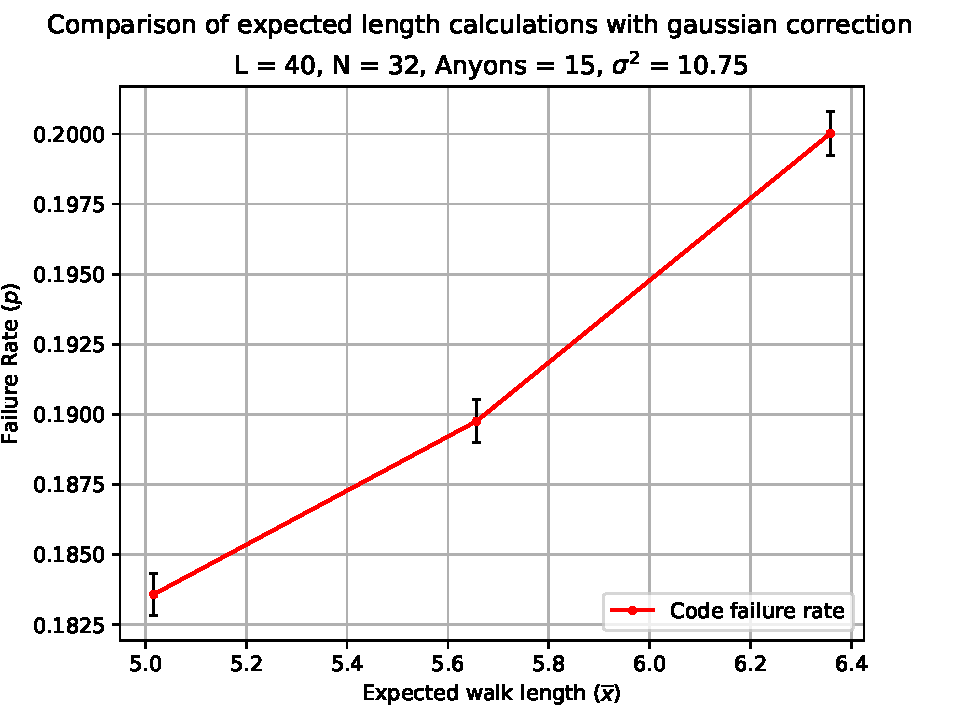
\includegraphics[width = 0.7\textwidth]{figs/comparison_of_methods}
	\caption{This trend clearly shows that the gaussian benefits from being centered at the expected walk length calculated from the pythagorean method of walk lengths. }
	\label{fig:methodcomparison}
\end{figure}
Figure \ref{fig:methodcomparison} is not conclusive in determining what is the optimal walk length to choose, however it does show that for the parameters used, the pythagorean distance gives the best success rate. All methods are more effective than the classical code, but pythag is best. \\
Obviously the next step is to run a higher accuracy scan over the 5.016 value, to determine if this is an accurate minimum, or just a coincidence. There is reason to believe that one of the three methods will be correlated to the best value for the mean; and that the best value, will be modulated from this calculation dependant upon the size of the code, and the anyon density, and the chain length. these `neighbour interactions' will likely dictate what the optimal parameters will be. This means that a practical implementation of the improved Toric code may require walking the parameters of the correction, until a global minimum of failure rate is found.  A good guess for the centre of the gaussian correction has however, been shown to any of the three expected walk length calculations; as all choices beat the classical code; for the current parameters. 

In the case of the gaussian, the centre of it may not even need to correspond exactly to one of the expected walk length calculations, as the gaussian is only approximating the actual walk length distribution of random walks. In the case where we correct using the actual distributions of random walks; we should see that it beats the gaussian for every parameter of the gaussian. 

The gamma functions however, may also need some degree of tuning to account for the `neighbour interactions'. 